\section{\label{sec:cumulants} Cumulants}
\subsection{Calculation of cumulants}
Let's calculate $\mathfrak{M}_n(\vb k_1, \dotsc, \vb k_n)$ based on Eqs.~(\ref{def:cumulant}),~(\ref{def:jacob_tilde}).
To simplify notation for the average value defined in~(\ref{def:average_rs}), the subscript $0$ will be used to indicate RS
$$ \langle \dotsc \rangle_0 \equiv \langle \dotsc \rangle_{RS} $$

For the first cumulant one gets:
\begin{equation}
	\label{m1_via_rho}
	\mathfrak{M}_1(\vb k) = \frac{1}{(-{\rm i}2\pi)} \frac{\partial \ln \tilde{\mathfrak{J}}(\omega)}{\partial \omega_{{\vb k}_1}} \bigg{|}_{\omega_{{\vb k}_i}=0} = \langle \hat{\rho}_{\vb k} \rangle_0
\end{equation}
For the second cumulant:
\begin{equation}
	\mathfrak{M}_2(\vb k_1, \vb k_2) = \frac{1}{(-{\rm i}2\pi)^2} \frac{\partial^2 \ln \tilde{\mathfrak{J}}(\omega)}{\partial \omega_{{\vb k}_1} \partial \omega_{{\vb k}_2}} \bigg{|}_{\omega_{{\vb k}_i}=0} 
	= \langle \hat{\rho}_{\vb k_1} \hat{\rho}_{\vb k_2} \rangle_0 - \langle \hat{\rho}_{\vb k_1} \rangle_0 \langle\hat{\rho}_{\vb k_2} \rangle_0
\end{equation}
Continuing this procedure, for the next cumulants one gets:
\begin{equation}
	\mathfrak{M}_3(\vb k_1, \vb k_2, \vb k_3) = 
	\langle \hat{\rho}_{\vb k_1} \hat{\rho}_{\vb k_2} \hat{\rho}_{\vb k_3} \rangle_0 
	- \sum_{\vb l = \left\{\substack{1,2,3 \\ 1,3,2 \\ 2,3,1}\right\}} 
	\langle \hat{\rho}_{\vb k_{l_1}} \hat{\rho}_{\vb k_{l_2}} \rangle_0 \langle \hat{\rho}_{\vb k_{l_3}} \rangle_0
	+ 2 \langle \hat{\rho}_{\vb k_1} \rangle_0 \langle\hat{\rho}_{\vb k_2} \rangle_0 \langle\hat{\rho}_{\vb k_3} \rangle_0
\end{equation}
\begin{eqnarray}
	\label{m4_via_rho}
	\mathfrak{M}_4(\vb k_1, \vb k_2, \vb k_3, \vb k_4) &=& 
	\langle \hat{\rho}_{\vb k_1} \hat{\rho}_{\vb k_2} \hat{\rho}_{\vb k_3} \hat{\rho}_{\vb k_4} \rangle_0 
	\nonumber\\
	&& - \sum_{\vb l = \left\{\substack{1,2,3,4 \\ 1,2,4,3 \\ 1,3,4,2 \\ 2,3,4,1}\right\}} 
	\langle \hat{\rho}_{\vb k_{l_1}} \hat{\rho}_{\vb k_{l_2}} \hat{\rho}_{\vb k_{l_3}} \rangle_0 \langle \hat{\rho}_{\vb k_{l_4}} \rangle_0
	-\sum_{\vb l = \left\{\substack{1,2,3,4 \\ 1,3,2,4 \\ 1,4,2,3 }\right\} } \langle \hat{\rho}_{\vb k_{l_1}} \hat{\rho}_{\vb k_{l_2}} \rangle_0 \langle \hat{\rho}_{\vb k_{l_3}} \hat{\rho}_{\vb k_{l_4}} \rangle_0 
	\nonumber\\
	&& +2 \sum_{\vb l = \left\{\substack{1,2,3,4 \\ 1,3,2,4 \\ 1,4,2,3 \\ 2,3,1,4 \\ 2,4,1,3 \\ 3,4,1,2 }\right\} } \langle \hat{\rho}_{\vb k_{l_1}} \hat{\rho}_{\vb k_{l_2}} \rangle_0 \langle\hat{\rho}_{\vb k_3} \rangle_0 \langle\hat{\rho}_{\vb k_4} \rangle_0
	\nonumber\\
	&& -6 \langle \hat{\rho}_{\vb k_1} \rangle_0 \langle\hat{\rho}_{\vb k_2} \rangle_0 \langle\hat{\rho}_{\vb k_3} \rangle_0 \langle\hat{\rho}_{\vb k_4} \rangle_0
\end{eqnarray}
The expressions in the right-hand sides of~(\ref{m1_via_rho})-(\ref{m4_via_rho}) can be called cumulant averages of $\hat{\rho}_{\vb k}$, since they remind formulae for cumulants expressed via non-central moments. In other words, if $\langle\rho_{\vb k_1} \dotsc \rho_{\bf k_n} \rangle$ are considered non-central moments (of a probability distribution), then $\mathfrak{M}_n(\vb k_1, \dotsc, \vb k_n)$ can be considered as cumulants (semi-invariants) and the relationships between them are known\cite{stuart2010kendall}.

As per our knowledge, the generic expression for cumulant average is not found so far, however, $\mathfrak{M}_n$ can be derived for any $n$ based on generating functional $\ln \tilde{\mathfrak{J}}(\omega)$ by virtue of~(\ref{def:cumulant}).

\subsection{\label{sec:cumulants_via_h} Cumulants $\mathfrak M_n(\vb k^n)$ expressed via Fourier components of the total correlation functions $\hat{h}^{(n)}(\vb k^n)$}
In this subsection, explicit expressions for cumulants $\mathfrak{M_n}$ are presented in terms of the Fourier components of total correlation functions $\hat{h}^{(n)}$. See Appendix~\ref{sec:total_corr_func} for the definition and some properties of total correlation functions. The calculation of the first two cumulants is presented in details in Appendix~\ref{app:cumulant_calc}.
\begin{equation}
\label{CumulantM1}
	\mathfrak M_1(\vb k) = \rho \hat{h}^{(1)}(\vb k) = \langle N \rangle_0 \delta_{\vb k}
\end{equation}

\begin{equation}
	\label{CumulantM2}
	\mathfrak M_2(\vb k_1, \vb k_2) = \rho \hat{h}^{(1)}(\vb k_1 + \vb k_2) + \rho^2\hat{h}^{(2)}(\vb k_1, \vb k_2) = \langle N \rangle_0 \delta_{\vb k_1 + \vb k_2} (1 + \rho \hat{h}^{(2)}(\vb k_1))
\end{equation}

\begin{eqnarray}
	\label{CumulantM3}
	\mathfrak M_3 (\vb k_1, \vb k_2, \vb k_3) &=& \rho \hat{h}^{(1)}(\vb k_1 + \vb k_2 + \vb k_3) \nonumber \\
	&&+ \rho^2(\hat{h}^{(2)}(\vb k_1 + \vb k_2, \vb k_3) + \hat{h}^{(2)}(\vb k_1 + \vb k_3, \vb k_2) + \hat{h}^{(2)}(\vb k_2 + \vb k_3, \vb k_1))  \nonumber \\
	&&+ \rho^3 \hat{h}^{(3)}(\vb k_1, \vb k_2, \vb k_3) 
	\nonumber \\
	&=& \rho \hat{h}^{(1)}(\vb k_1 + \vb k_2 + \vb k_3) + 
	\rho^2 \sum_{{\vb l}=\left\{ \substack{1,2,3 \\ 1,3,2 \\ 2,3,1}
 		\right\}}
	\hat{h}^{(2)}(\vb k_{l_1} + \vb k_{l_2}, \vb k_{l_3})
	+ \rho^3 \hat{h}^{(3)}(\vb k_1, \vb k_2, \vb k_3)
	\nonumber \\
	&=& \rho \hat{h}^{(1)}(\vb k_1 + \vb k_2 + \vb k_3) + 
	\rho^2 \sum_{\left\{3 \right\}}
	\hat{h}^{(2)}(\vb k_{l_1} + \vb k_{l_2}, \vb k_{l_3})
	+ \rho^3 \hat{h}^{(3)}(\vb k_1, \vb k_2, \vb k_3)
	\nonumber \\
	&=& \langle N \rangle_0 \delta_{\vb k_1 + \vb k_2 + \vb k_3} 
	\left[ 1 + \rho(\hat{h}^{(2)}(\vb k_1) + \hat{h}^{(2)}(\vb k_2) + \hat{h}^{(2)}(\vb k_1 + \vb k_2)) )\right. \nonumber\\
	&& \left. + \rho^2 \hat{h}^{(3)}(\vb k_1, \vb k_2) \right]
\end{eqnarray}

\begin{eqnarray}
	\label{CumulantM4}
	\mathfrak M_4 (\vb k_1, \dotsc, \vb k_4) &=& \rho \hat{h}^{(1)}(\vb k_1 + \dotsc + \vb k_4) 
	\nonumber\\
	&& + \rho^2 \sum_{\vb l = \left\{ \substack{1,2,3,4 \\ 1,2,4,3 \\ 1,3,4,2 \\ 2,3,4,1} \right\}}
	\hat{h}^{(2)}(\vb k_{l_1} + \vb k_{l_2} + \vb k_{l_3}, \vb k_{l_4})
	\nonumber\\
	&& + \rho^2
	\sum_{\vb l = \left\{ \substack{1,2,3,4 \\ 1,3,2,4 \\ 1,4,2,3} \right\}}
	\hat{h}^{(2)}(\vb k_{l_1} + \vb k_{l_2}, \vb k_{l_3} + \vb k_{l_4})
	\nonumber\\
	&& + \rho^3
	\sum_{\vb l = \left\{\substack{1,2,3,4 \\ 1,3,2,4 \\ 1,4,2,3 \\ 2,3,1,4 \\ 2,4,1,3 \\ 3,4,1,2} \right\} }
	\hat{h}^{(3)}(\vb k_{l_1} + \vb k_{l_2}, \vb k_{l_3}, \vb k_{l_4})
	\nonumber\\
	&& +\rho^4 \hat{h}^{(4)}(\vb k_1, \dotsc, \vb k_4)
	\nonumber \\
	&=& \langle N \rangle_0 \delta_{\vb k_1 + \vb k_2 + \vb k_3 + \vb k_4} 
	\left[ 1 + \rho\sum_{l = 1}^4 \hat{h}^{(2)}(\vb k_l) + 
	\rho 
	\sum_{\vb l = \left\{\substack{1,2 \\ 1,3 \\ 1,4}\right\}}
	\hat{h}^{(2)} (\vb k_{l_1} + \vb k_{l_2})
	\right. \nonumber \\
	&& \left. + \rho^2
	\sum_{\vb l = \left\{\substack{3,4 \\ 2,4 \\ 2,3 \\ 1,4 \\ 1,3 \\ 1,2}\right\} }
	\hat{h}^{(3)}(\vb k_{l_1}, \vb k_{l_2})
	+ \rho^3 \hat{h}^{(4)} (\vb k_1, \vb k_2, \vb k_3)
	\right] 
\end{eqnarray}

The expression in the square brackets next to the $\delta$-function for $\mathfrak M_4(\vb k^n)$ can be also written in a form where it depends only on $\vb k_1, \vb k_2, \vb k_3$, but does not depend on $\vb k_4$.
Let's write for $\mathfrak M_4$:

\begin{equation}
\mathfrak M_4(\vb k_, \dotsc, \vb k_4) = \langle N \rangle_0 \delta_{\vb k_1 + \vb k_2 + \vb k_3 + \vb k_4} \mathfrak m_4(\vb k_1, \vb k_2, \vb k_3) 
\end{equation}
Then
\begin{eqnarray}
	\label{m4}
	\mathfrak m_4(\vb k_1, \vb k_2, \vb k_3) &=&  1 + \rho \bigg(
	\sum_{l = 1}^3 \hat{h}^{(2)}(\vb k_l) +
	\sum_{\vb l = \left\{\substack{1,2 \\ 1,3 \\ 2,3} \right\} }  \hat{h}^{(2)} (\vb k_{l_1} + \vb k_{l_2})
	+ \hat{h}^{(2)} (\vb k_1 + \vb k_2 + \vb k_3)
	\bigg)
	\nonumber \\
	&&  + \rho^2 \bigg(
	\sum_{\vb l = \left\{\substack{1,2 \\ 1,3 \\ 2,3 }\right\} }
	\hat{h}^{(3)}(\vb k_{l_1}, \vb k_{l_2})
	+ \sum_{\vb l = \left\{\substack{1,2,3 \\ 1,3,2 \\ 2,3,1}\right\} }
	\hat{h}^{(3)}(\vb k_{l_1} + \vb k_{l_2}, \vb k_{l_3})
	\bigg)
	\nonumber\\
	&& + \rho^3 \hat{h}^{(4)} (\vb k_1, \vb k_2, \vb k_3)
\end{eqnarray}


This should be true for any $n$: a cumulant $\mathfrak M_n$ can be written in such a way, that dependence on $\vb k_n$ will be present only in $\delta_{\vb k_1 + \dotsc + \vb k_n}$, and other part, let's denote it by $\mathfrak m_n$, will depend only on $\vb k_1, \dotsc, \vb k_{n-1}$, or $\mathfrak m_n = \mathfrak m_n(\vb k^{n-1})$
\begin{equation}
	\mathfrak M_n(\vb k^n) = \langle N \rangle_0 \delta_{\vb k_1 + \dotsc + \vb k_n} \mathfrak m_n(\vb k^{n-1}).
\end{equation}
A few first $\mathfrak m_n$ are expressed via total correlation functions $\hat{h}^{(n)}$ as follows:
\begin{equation}
	\mathfrak{m}_1 = 1.
\end{equation}
\begin{equation}
	\label{m2}
	\mathfrak m_2(\vb k) = 1 + \rho \hat{h}^{(2)}(\vb k).
\end{equation}
\begin{equation}
	\label{m3}
	\mathfrak m_3(\vb k_1, \vb k_2) = 1 +  \rho \big(\hat{h}^{(2)}(\vb k_1) + \hat{h}^{(2)}(\vb k_2) + \hat{h}^{(2)}(\vb k_1 + \vb k_2) \big) 
	+ \rho^2 \hat{h}^{(3)}(\vb k_1, \vb k_2)
\end{equation}
and the expression for $\mathfrak m_4$ is given by~(\ref{m4}).
It is seen from~(\ref{m2}) that $\mathfrak m_2(\vb k)$ is the structure factor (see e.g Eq.~(3.6.10) in~\cite{HANSEN2013ch3}). By analogy, $\mathfrak{m}_n$ can be considered as the $n$-particle structure factor.

Expressions~(\ref{CumulantM1})-(\ref{CumulantM4}) for cumulants obtained in this work can be compared with corresponding expressions presented in other works.
In~\cite{YukhJSP1995} (see Appendix B therein), and in~\cite{Idzik1987En} (see Eq.~(3.7) therein), the expressions for $\mathfrak{M}_2$ through $\mathfrak{M}_4$ were presented in a similar form, but different permutations of wave-vector values were not accounted for. For example, it was considered that $\hat{h}^{(2)}(\vb k_1) + \hat{h}^{(2)}(\vb k_2) + \hat{h}^{(2)}(\vb k_1 + \vb k_2) = 3\hat{h}^{(2)}(\vb k_1)$.
In~\cite{Yukh1989tmpEn} (see Eqs.~(2.6), (2.10), and (2.11) therein), the expressions for $\mathfrak{M}_n(\vb k^n)$ were presented in a more complicated form, possibly due to the fact that correlation functions were defined in the canonical ensemble.

In~\cite{Pats1990tmf} the expressions analogous to~(\ref{CumulantM1})-(\ref{CumulantM4}) were written for cumulants of multicomponent system.


[NOTE: Need to verify the generic formula for $\mathfrak M_n$, see e.g., Eq.~(2.12) in~\cite{Yukh1990}, Eq.~(2.4) in~\cite{Yukh1989tmpEn}, and Eq.~(3.6) in ~\cite{Idzik1987En}]

There are a few interesting properties to note about general expression for $\mathfrak{m_n}$. First, that the number of all terms contributing to $\mathfrak{m_n}$ is equal to the Bell number $B_n$\cite{cameron1995comb,wikiBellNum}. Second, if the terms are grouped by the powers in $\rho$ then the number of terms at the $k$-th power in $\rho$ is the Stirling number of the second kind $S(n,k)$\cite{cameron1995comb,wikiStirlingNum2}.

\subsection{Explicit expressions for cumulants as functions of wave-vector and packing fraction}
To start with, one can use an explicit equation for the structure factor of hard-spheres system. For example, let's use Eq.~(3) from~\cite{Ashcroft1966} for the structure factor as a function of wave-vector and packing fraction $\eta$ in the Percus-Yevick approximation
\begin{equation}
	\mathfrak{M}_2(\vb k, -\vb k)/\langle N \rangle_0 = \mathfrak{m}_2(\vb k),
\end{equation}
\begin{equation}
	\mathfrak{m}_2(k) = (1 - \rho c(k))^{-1},
\end{equation}
where $c(k)$ is the Fourier component of the direct correlation function:
\begin{equation}
	c(k) = -4\pi\sigma^3\int_{0}^{1} {\rm d} s s^2 \frac{\sin(s k \sigma)}{s k \sigma} (A + Bs +Cs^3)
\end{equation}
The parameters $A$, $B$, and $C$ are functions of $\eta$:
\begin{eqnarray}
 A = (1+2\eta)^2/(1-\eta)^4 
 \nonumber\\
 B = -6\eta(1+\eta/2)^2/(1-\eta)^4
 \nonumber\\
 C = (1/2)\eta(1+2\eta)^2/(1-\eta)^4.
\end{eqnarray}
In Figure~\ref{m2_vs_k} $\mathfrak{m}_2$ is shown as a function of $k\cdot\sigma$ at different values of $\eta$. In Figure~\ref{m2_vs_eta} $\mathfrak{m}_2$ is shown as a function of $\eta$ at $k=0$.

\begin{figure}[htbp]
	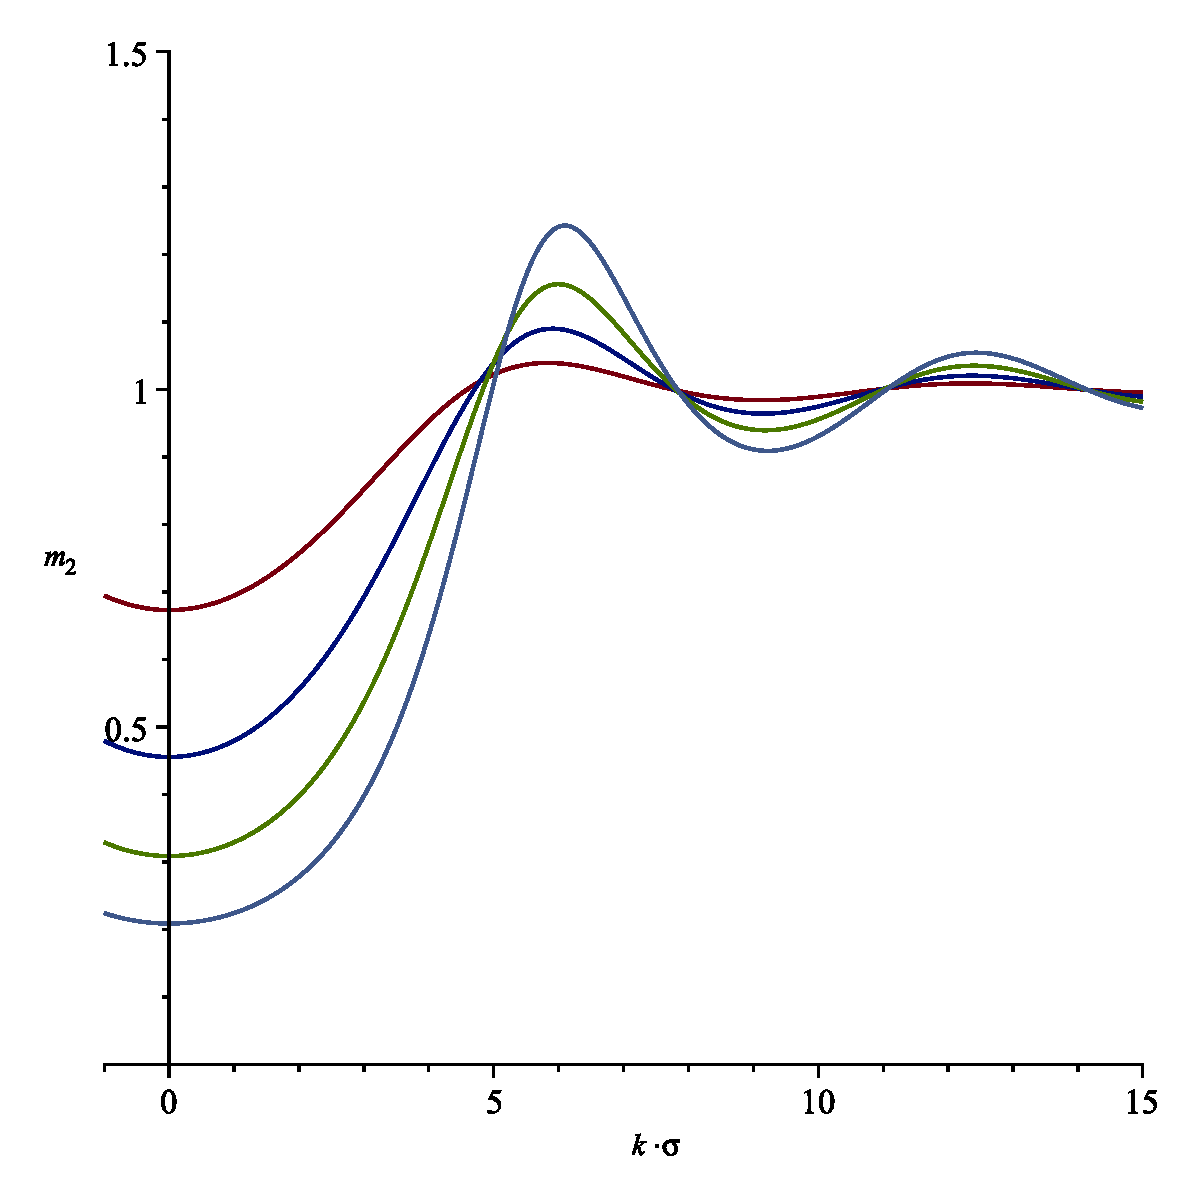
\includegraphics[width=0.45\textwidth,angle=0]{M2_as_function_of_k_at_different_eta} \hfill
	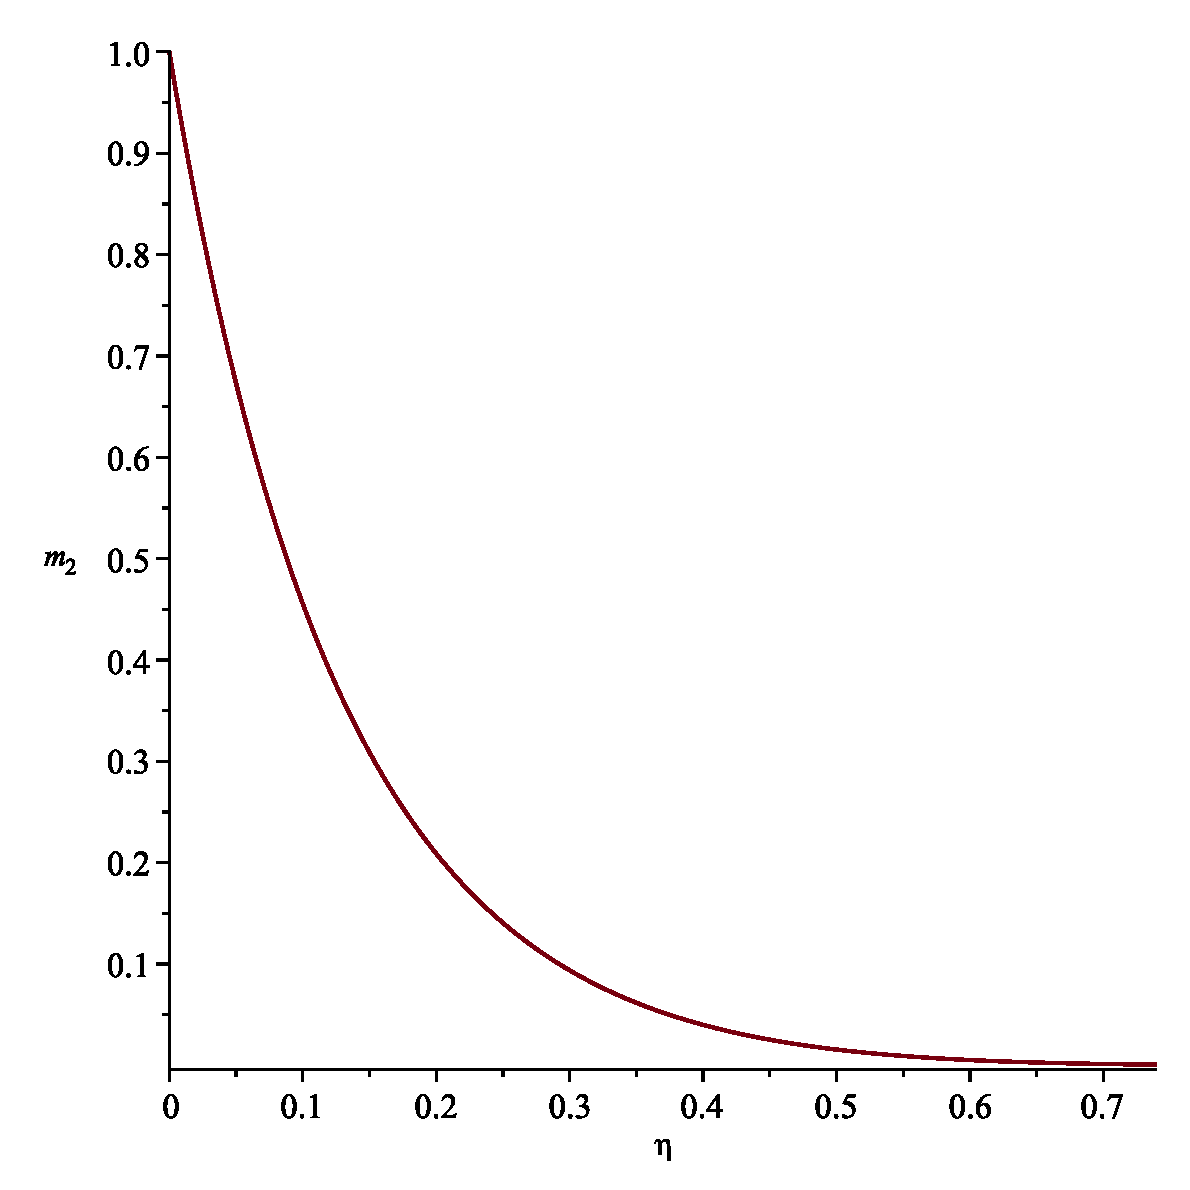
\includegraphics[width=0.45\textwidth,angle=0]{M2_as_function_of_eta_at_k_equals_0} \\
	\parbox{0.5\textwidth}{\caption{\label{m2_vs_k} Cumulant $\mathfrak{m}_2$ as a function of $k\sigma$ at different values of packing fraction $\eta$. $\eta = 0.05$, $\eta=0.1$, $\eta = 0.15$, and $\eta=0.2$.
	}} \hfill
	\parbox{0.45\textwidth}{\caption{\label{m2_vs_eta} Cumulant $\mathfrak{m}_2$ as a function of packing fraction $\eta$ at $\vb k = 0$
	}}
\end{figure}

The formulas for $\mathfrak{M}_3(\vb k, -\vb k, 0)$ and $\mathfrak{M}_4(\vb k, -\vb k, 0, 0)$ can be obtained from $\mathfrak{M}_2(\vb k, -\vb k)$ based on the recurrence relations for $n$-particle distribution functions $g_n$ found in~\cite{Schofield1966} (see Eq.~(A8) therein). Such formulas were obtained in~\cite{YukhJSP1995} (see Appendix B therein) and in our notation they read:
\begin{equation}
	\label{recur_m3_m2}
	\mathfrak{m}_3(\vb k, -\vb k) = \mathfrak{m}_2(0) 
	\left[
		\mathfrak{m}_2(\vb k) + \eta\frac{\partial\mathfrak{m}_2(\vb k)}{\partial\eta}
	\right],
\end{equation}

\begin{eqnarray}
	\label{recur_m4_m2}
	\mathfrak{m}_4(k, -k, 0) &=& \mathfrak{m}_2(0) 
	\left[
		\mathfrak{m}_2(k)\mathfrak{m}_2(0) + 3\eta\mathfrak{m}_2(0)\frac{\partial\mathfrak{m}_2(k)}{\partial\eta}
	\right.
	\nonumber\\
	&& \left. 
	+ \eta\mathfrak{m}_2(k)\frac{\partial\mathfrak{m}_2(0)}{\partial\eta} 
	+ \eta^2\frac{\partial\mathfrak{m}_2(0)}{\partial\eta} \frac{\partial\mathfrak{m}_2(k)}{\partial\eta}
	+ \eta^2\mathfrak{m}_2(0)\frac{\partial^2\mathfrak{m}_2(k)}{\partial\eta^2}
	\right]
\end{eqnarray}

\begin{figure}[htbp]
	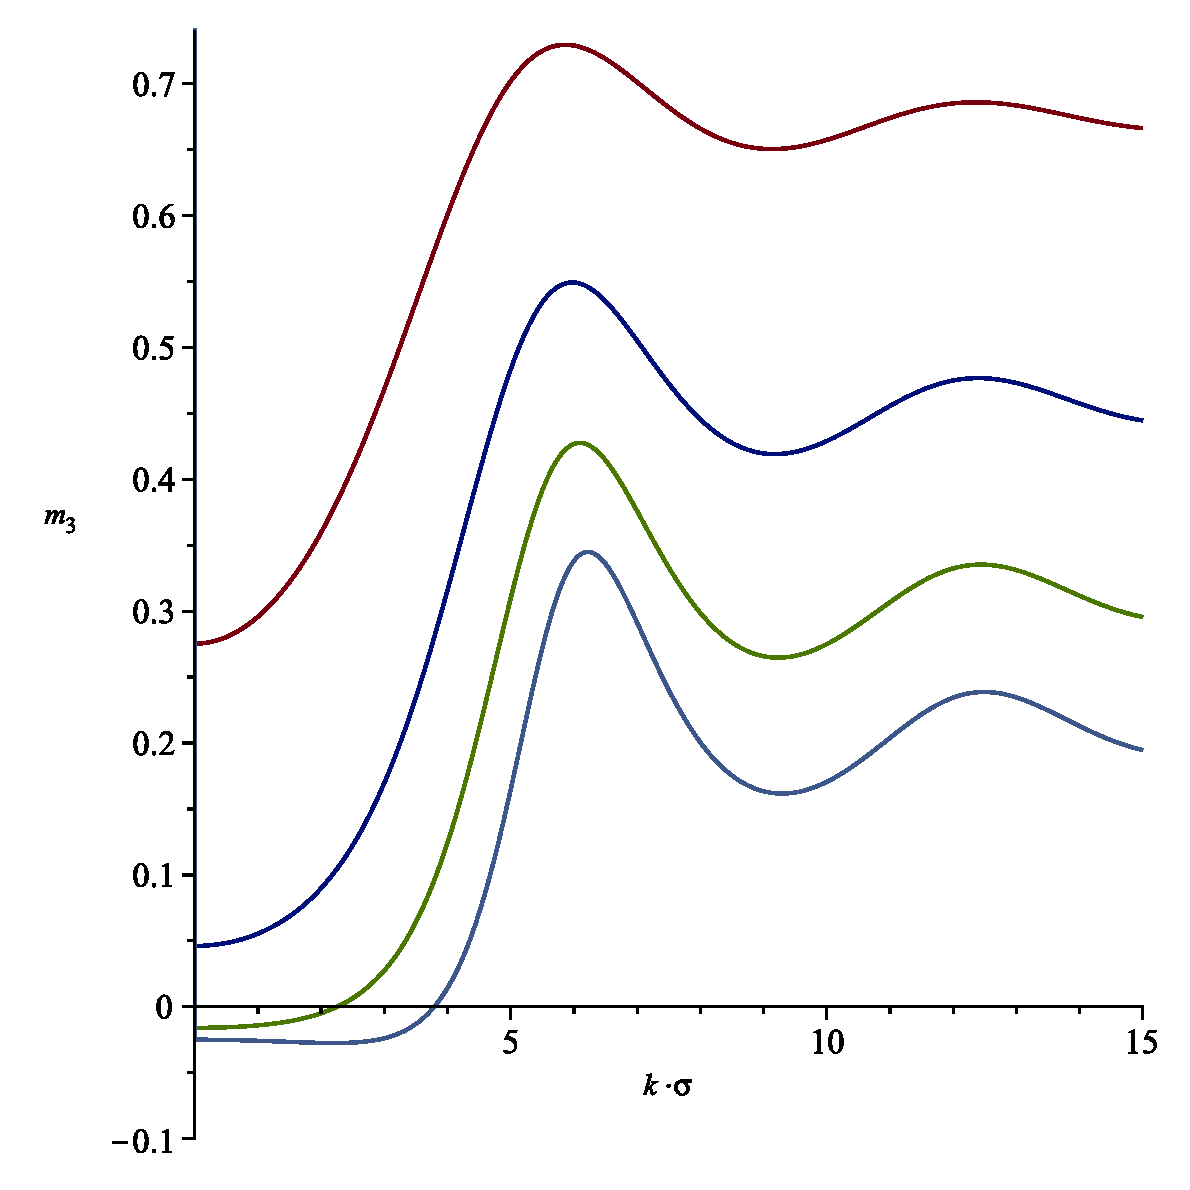
\includegraphics[width=0.45\textwidth,angle=0]{M3_as_function_of_k_at_different_eta} \hfill
	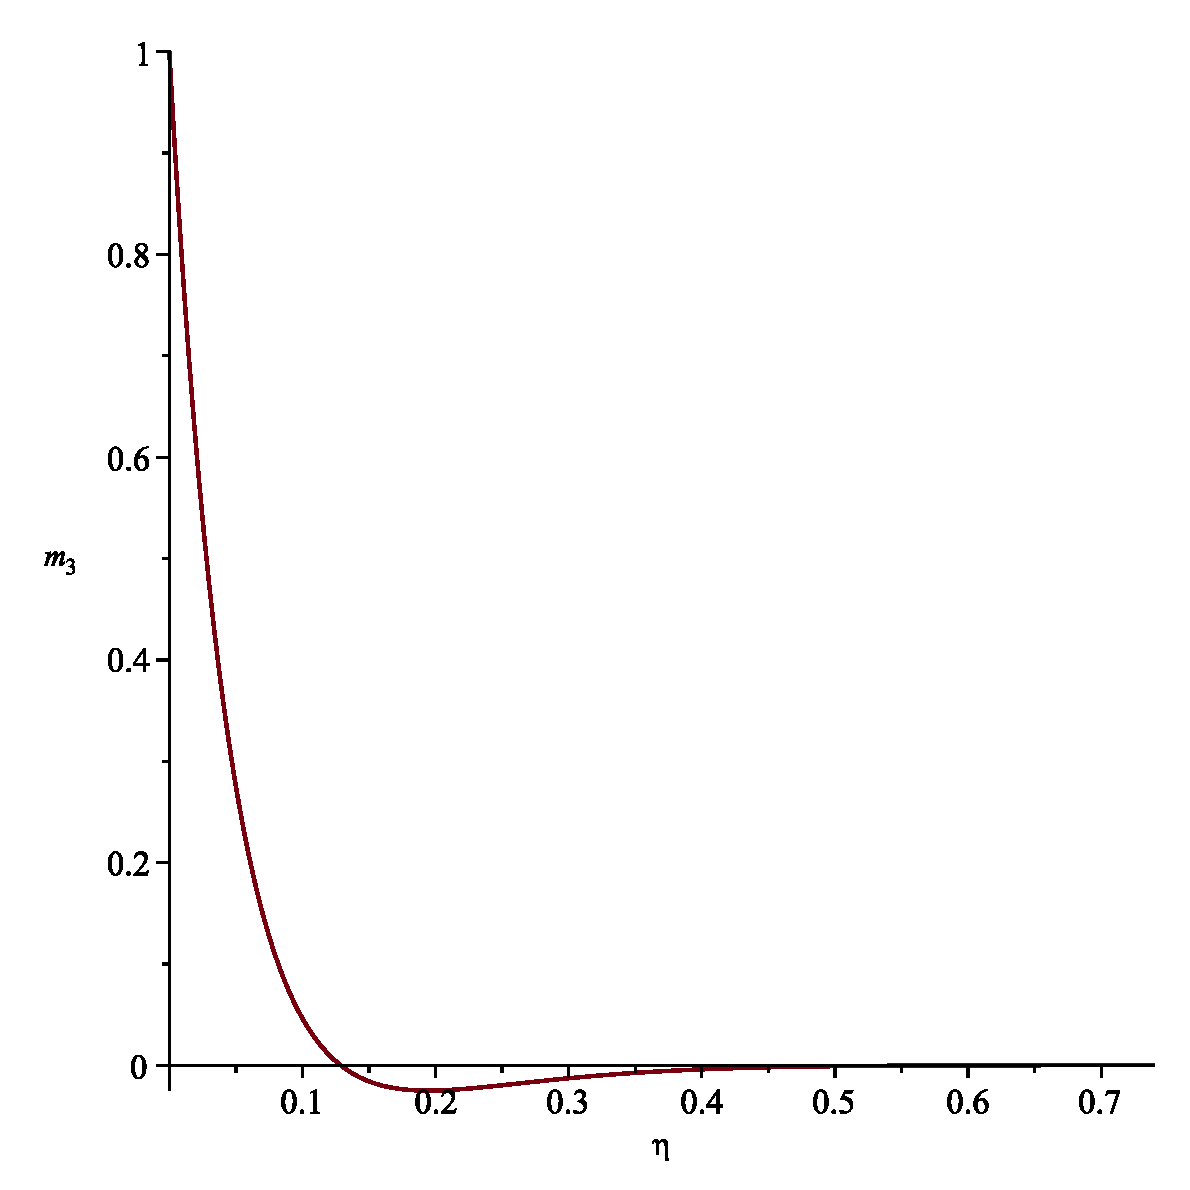
\includegraphics[width=0.45\textwidth,angle=0]{M3_as_function_of_eta_at_k_equals_0} \\
	\parbox{0.5\textwidth}{\caption{\label{m3_vs_k} Cumulant $\mathfrak{m}_3$ as a function of $k\sigma$ at different values of packing fraction $\eta$. $\eta = 0.05$, $\eta=0.1$, $\eta = 0.15$, and $\eta=0.2$.
	}} \hfill
	\parbox{0.45\textwidth}{\caption{\label{m3_vs_eta} Cumulant $\mathfrak{m}_3$ as a function of packing fraction $\eta$ at $\vb k = 0$
	}}
\end{figure}
\begin{figure}[htbp]
	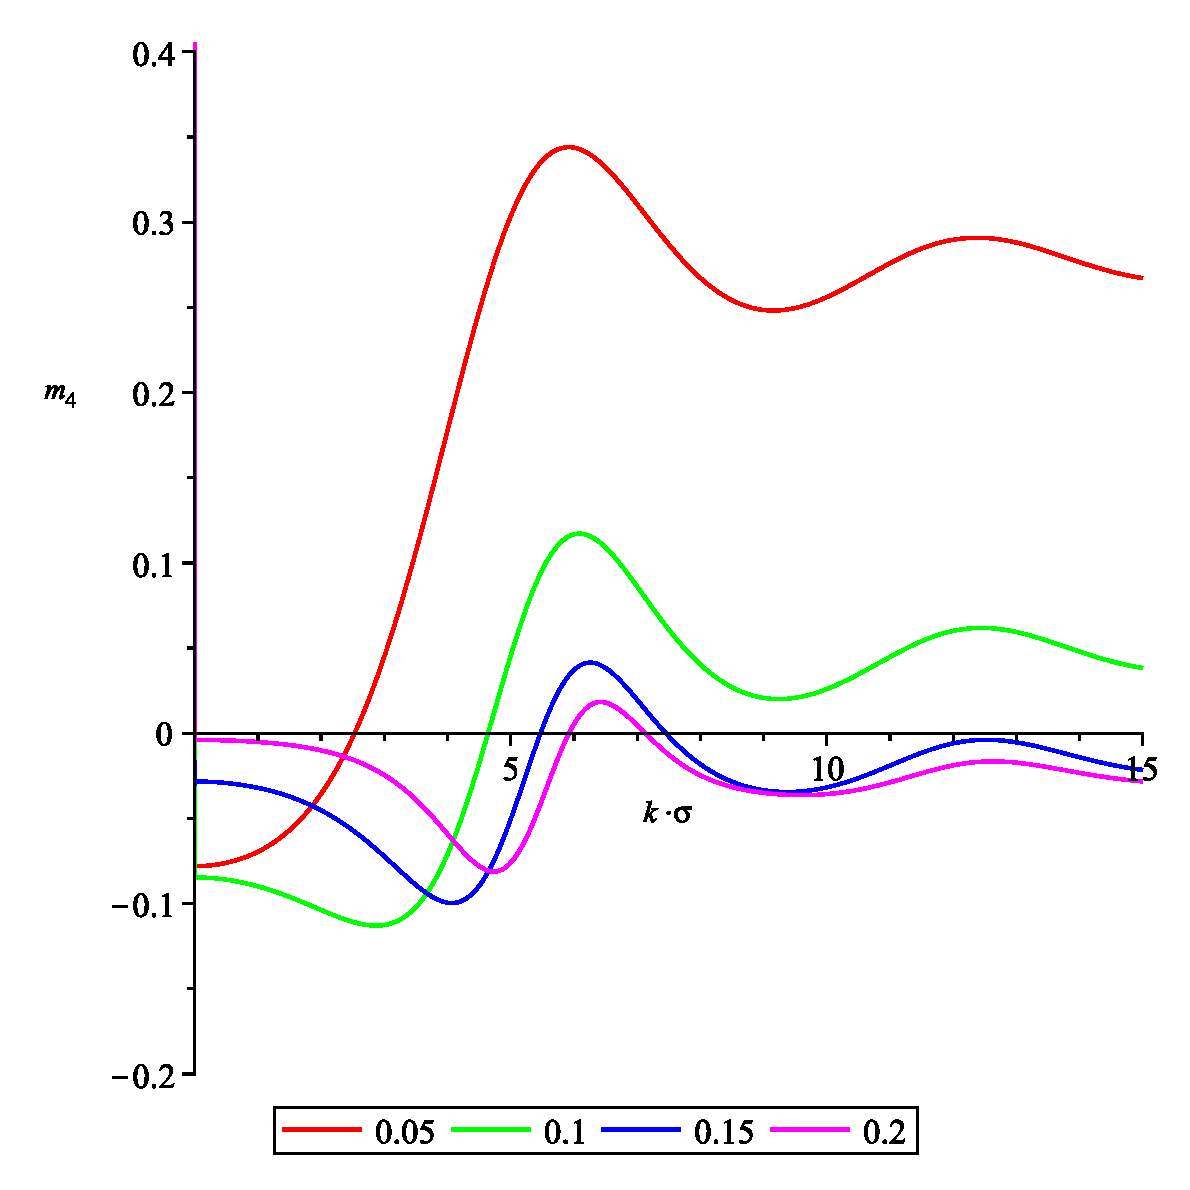
\includegraphics[width=0.45\textwidth,angle=0]{M4_as_function_of_k_at_different_eta} \hfill
	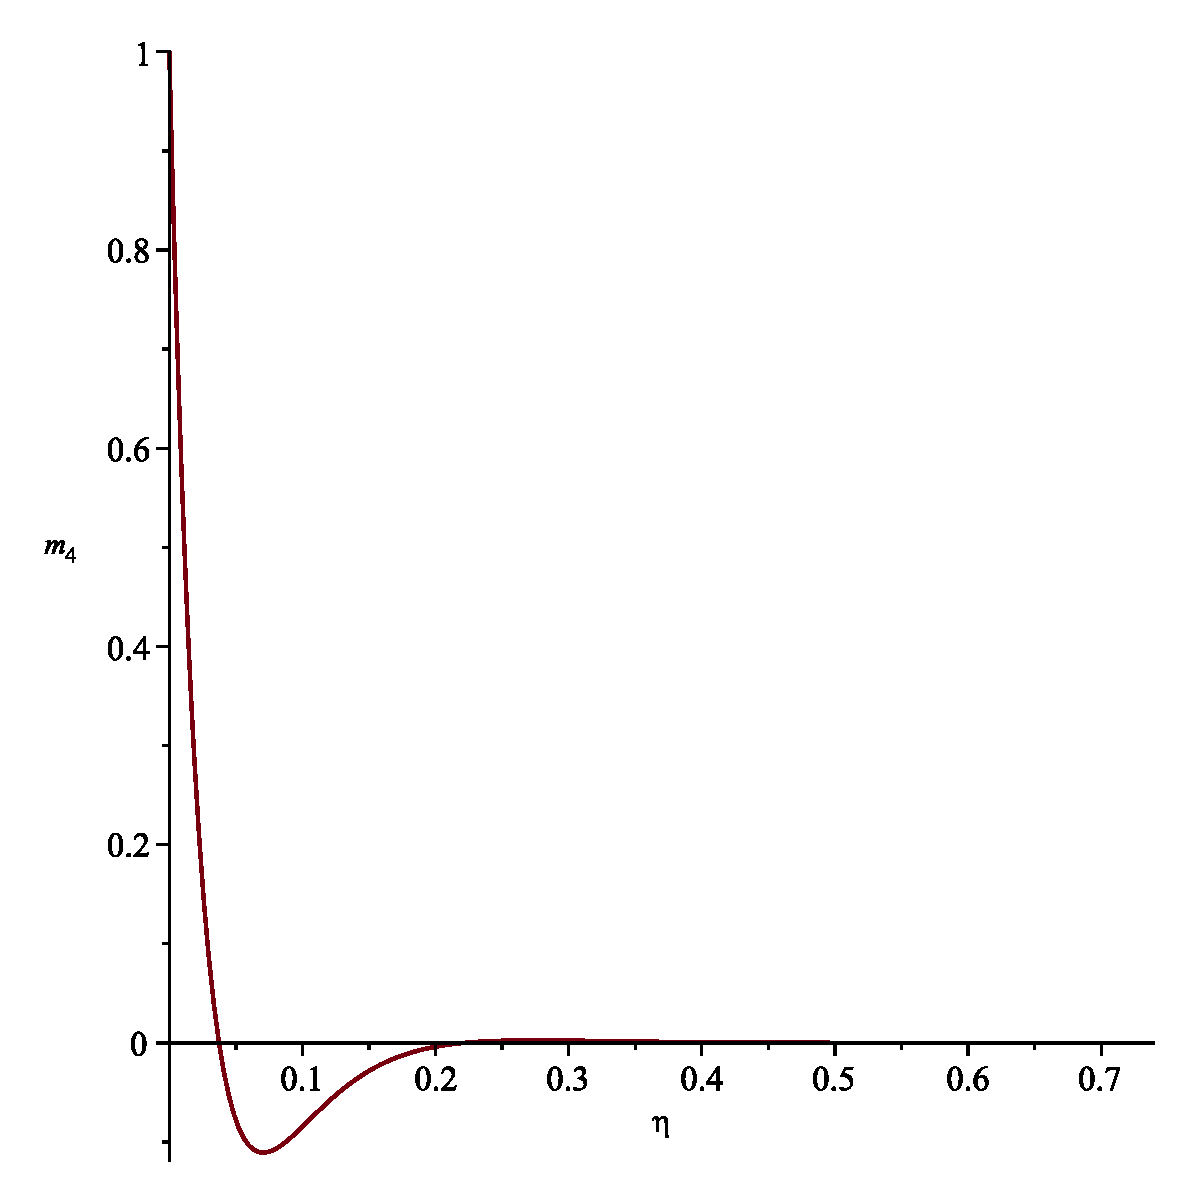
\includegraphics[width=0.45\textwidth,angle=0]{M4_as_function_of_eta_at_k_equals_0} \\
	\parbox{0.5\textwidth}{\caption{\label{m4_vs_k} Cumulant $\mathfrak{m}_4$ as a function of $k\sigma$ at different values of packing fraction $\eta$. $\eta = 0.05$, $\eta=0.1$, $\eta = 0.15$, and $\eta=0.2$.
	}} \hfill
	\parbox{0.45\textwidth}{\caption{\label{m4_vs_eta} Cumulant $\mathfrak{m}_4$ as a function of packing fraction $\eta$ at $\vb k = 0$
	}}
\end{figure}
In Figure~\ref{m3_vs_k} $\mathfrak{m}_3$ is shown as a function of $k\cdot\sigma$ at different values of $\eta$. In Figure~\ref{m3_vs_eta} $\mathfrak{m}_3$ is shown as a function of $\eta$ at $k=0$.
In Figure~\ref{m4_vs_k} $\mathfrak{m}_4$ is shown as a function of $k\cdot\sigma$ at different values of $\eta$. In Figure~\ref{m4_vs_eta} $\mathfrak{m}_4$ is shown as a function of $\eta$ at $k=0$.

\subsection{Cumulants at $\vb k_i = 0$}
At $\vb k_i = 0$ cumulants are expressed via the average number of particles in the reference system.
Here the final expressions are presented. They are obtained directly from~(\ref{m1_via_rho})--(\ref{m4_via_rho}) by substituting $\vb k_i=0$ and using $\hat{\rho}_0 = N$. Some alternative methods to calculate them are presented in Appendix~\ref{app:cumulant_calc_k_0}.
\begin{equation}
	\mathfrak{M}_1(0) = \langle N \rangle_0;
\end{equation}

\begin{equation}
	\mathfrak{M}_2(0,0) = \langle N^2 \rangle_0 - \langle N \rangle_0^2 = \langle (N - \langle N \rangle_0)^2 \rangle_0;
\end{equation}

\begin{eqnarray}
	\mathfrak{M}_3(0,0,0) &=& \langle N^3 \rangle_0 - 3 \langle N^2 \rangle_0 \langle N \rangle_0 +2\langle N \rangle_0^3
	\nonumber\\
	&=& \langle (N - \langle N \rangle_0)^3 \rangle_0;
\end{eqnarray}

\begin{eqnarray}
	\mathfrak{M}_4(0,0,0,0) &=& \langle N^4 \rangle_0 
	- 4\langle N^3 \rangle_0\langle N \rangle_0 
	+ 12\langle N^2 \rangle_0\langle N \rangle_0^2 
	- 3\langle N^2 \rangle_0^2 
	- 6\langle N \rangle_0^4
	\nonumber\\
	&=& \langle (N - \langle N \rangle_0)^4 \rangle_0 - 3 \langle (N - \langle N \rangle_0)^2 \rangle_0^2.
\end{eqnarray}

\subsection{Cumulants as functions of packing fraction for the hard-spheres system}
For the system of hard spheres the cumulants $\mathfrak{m}_n$ can be found explicitly as functions of the packing fraction $\eta$ based on a given equation of state
\begin{equation}
	\frac{PV}{NkT} = f(\eta)
\end{equation}
where $f(\eta)$ is a function of the packing fraction only. The structure factor at zero wave-vector value is found via
\begin{equation}
	\mathfrak{m}_2 = S(0) = kT\left(\frac{\partial \rho}{\partial P}\right)_T.
\end{equation}
From here one has
\begin{equation}
	\frac{1}{\mathfrak{m}_2} = f(\eta) + \eta \frac{\partial f(\eta)}{\partial \eta}.
\end{equation}
For example, in~\cite{Idzik1987En}, the following expressions were obtained based on the equation of state by Carnahan and Starling~\cite{CarnahanStarling1969} for HS:
\begin{equation}
	\mathfrak{m}_2 = \frac{(1-\eta)^4}{(1+2\eta)^2 - 4\eta^3 + \eta^4},
\end{equation}
\begin{equation}
	\mathfrak{m}_3 = \frac{(1-\eta)^7(1 - 5\eta - 20\eta^2 - 4\eta^3 + 5\eta^4 - \eta^5)}{((1+2\eta)^2 - 4\eta^3 + \eta^4)^3},
\end{equation}
\begin{eqnarray}
	\mathfrak{m}_4 &=& (1-\eta)^{10}(1 - 26 \eta - 35\eta^2 + 408\eta^3 + 758\eta^4 + 28\eta^5 -
	\nonumber\\
	&&-114\eta^6 - 40\eta^7 + 37\eta^8 - 10\eta^9 + \eta^{10}) ((1+2\eta)^2 - 4\eta^3 + \eta^4)^{-5}.
\end{eqnarray}
Note that here the signs for the term $4\eta^3$ in $\mathfrak{m}_3$ and for $408\eta^3$ in $\mathfrak{m}_4$ were corrected.
